\documentclass[12pt, a4paper]{article}

% ─── Packages ──────────────────────────────────────────────────────────────
\usepackage[utf8]{inputenc}
\usepackage[T1]{fontenc}
\usepackage{lmodern}
\usepackage[margin=1in]{geometry}
\usepackage{graphicx}
\usepackage{float}
\usepackage{hyperref}
\usepackage{xcolor}
\usepackage{titlesec}
\usepackage{fancyhdr}
\usepackage{enumitem}
\usepackage{tabularx}
\usepackage{booktabs}
\usepackage{caption}
\usepackage{subcaption}
\usepackage{parskip}

% ─── Colors ────────────────────────────────────────────────────────────────
\definecolor{primaryblue}{RGB}{30, 58, 138}
\definecolor{accentblue}{RGB}{59, 130, 246}
\definecolor{darkgray}{RGB}{40, 40, 40}

% ─── Hyperref Setup ────────────────────────────────────────────────────────
\hypersetup{
    colorlinks=true,
    linkcolor=primaryblue,
    urlcolor=accentblue,
    citecolor=primaryblue,
    pdftitle={Docker Hands-On Lab Assignment Report},
    pdfauthor={Neel Prajapati},
}

% ─── Header/Footer ────────────────────────────────────────────────────────
\pagestyle{fancy}
\fancyhf{}
\fancyhead[C]{\small\textit{Docker Hands-On Lab Assignment | Neel Prajapati (202611022)}}
\fancyfoot[C]{\thepage}
\renewcommand{\headrulewidth}{0.4pt}
\renewcommand{\footrulewidth}{0.4pt}

% ─── Section Styling ──────────────────────────────────────────────────────
\titleformat{\section}{\Large\bfseries\color{primaryblue}}{}{0em}{}
\titleformat{\subsection}{\large\bfseries\color{accentblue}}{}{0em}{}

% ─── Graphics Path ─────────────────────────────────────────────────────────
\graphicspath{{images/}}

% ═══════════════════════════════════════════════════════════════════════════
\begin{document}

% ─── TITLE PAGE ────────────────────────────────────────────────────────────
\begin{titlepage}
    \centering
    \vspace*{1cm}

    {\color{primaryblue}\rule{\linewidth}{2pt}}
    \vspace{0.5cm}

    {\large Subject: Cloud Computing (CC)}\\[1.5cm]

    {\Huge\bfseries\color{primaryblue} Docker Hands-On\\Lab Assignment}\\[0.5cm]
    {\large A 2-Hour Hands-On Lab: Containers, Images, Dockerfiles \& Registries}

    \vspace{2cm}

    \fbox{
        \begin{minipage}{0.6\textwidth}
            \centering
            \vspace{0.5cm}
            {\Large\bfseries\color{primaryblue} Neel Prajapati}\\[0.3cm]
            {\large Enrollment No: 202611022}\\[0.5cm]
        \end{minipage}
    }

    \vfill

    {\small\textit{Lab Reference: \url{https://techifylabs-docker.learnwithdutta.com/}}}

    \vspace{1cm}
    {\color{primaryblue}\rule{\linewidth}{2pt}}
\end{titlepage}

% ─── TABLE OF CONTENTS ────────────────────────────────────────────────────
\tableofcontents
\newpage

% ═══════════════════════════════════════════════════════════════════════════
\section{Introduction}

This report documents the Docker Hands-On Lab Assignment completed as part of the Cloud Computing (CC) course. The lab consists of nine carefully structured steps designed to provide practical, hands-on experience with Docker containers, images, Dockerfiles, volumes, and container registries.

The lab was conducted following the instructions provided at \url{https://techifylabs-docker.learnwithdutta.com/}. The objective was to understand containerization concepts through direct experimentation --- running containers, examining their internals, building custom images, managing persistent data, and deploying production-ready containers.

\textbf{Key concepts covered include:}
\begin{itemize}[nosep]
    \item Containers vs Virtual Machines
    \item Docker architecture (CLI, daemon, containerd, shim, runc)
    \item Namespaces and cgroups for isolation and resource limits
    \item Image layers and copy-on-write filesystem
    \item Dockerfile best practices (layer ordering, exec-form ENTRYPOINT)
    \item Docker volumes for persistent storage
    \item Multi-stage builds, non-root users, and health checks
    \item Container registries for image distribution
\end{itemize}

% ═══════════════════════════════════════════════════════════════════════════
\section{Setup Check}

Checking Docker Desktop installation --- encountered a virtualization support error on Windows. This prompted setting up Docker via WSL2 instead.

\begin{figure}[H]
    \centering
    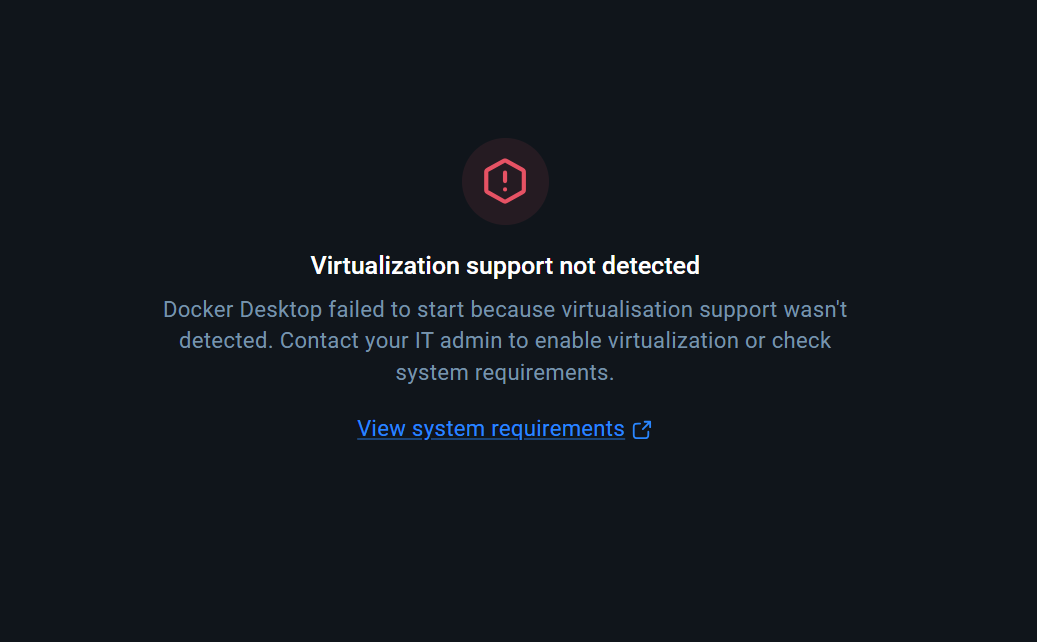
\includegraphics[width=0.85\textwidth]{Screenshot 2026-09-30 122327.png}
    \caption{Docker Desktop --- Virtualization support not detected}
\end{figure}

% ═══════════════════════════════════════════════════════════════════════════
\section{Step 1: Run Your First Container}

\subsection{Docker Installation Check in WSL2}

Attempting to run Docker commands in WSL2. Initially, Docker was not found in the WSL2 distro, requiring manual installation of Docker Engine inside Ubuntu.

\begin{figure}[H]
    \centering
    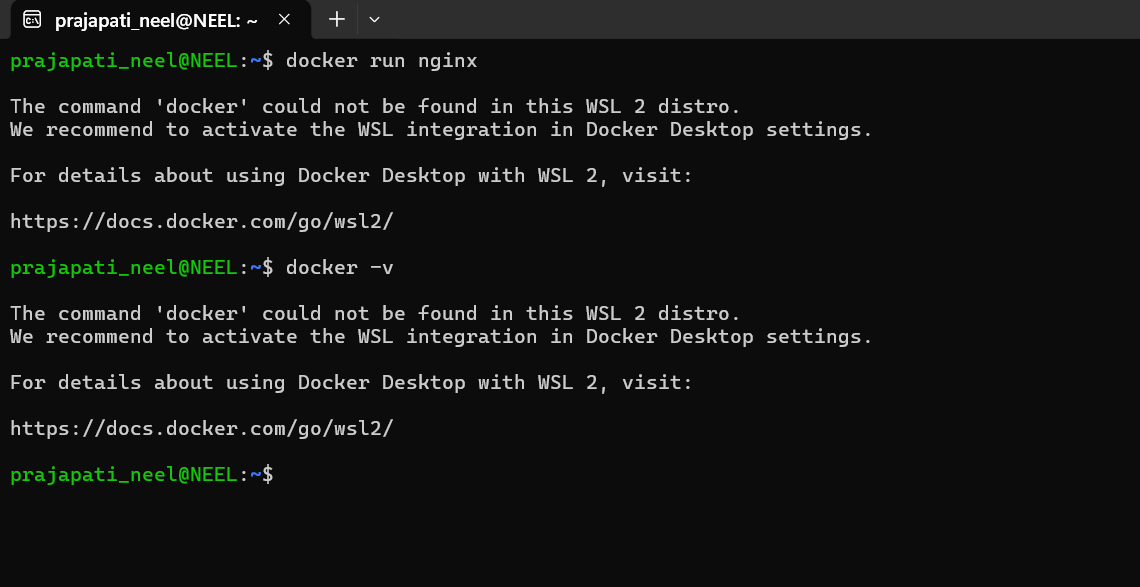
\includegraphics[width=0.85\textwidth]{Screenshot 2026-09-30 131745.png}
    \caption{Docker not found in WSL2 --- installing Docker Engine}
\end{figure}

\subsection{Running First Nginx Container}

After installing Docker Engine in WSL2, successfully ran the first Nginx container using \texttt{docker run -d --name web -p 8080:80 nginx:alpine} and verified it with \texttt{curl}.

\begin{figure}[H]
    \centering
    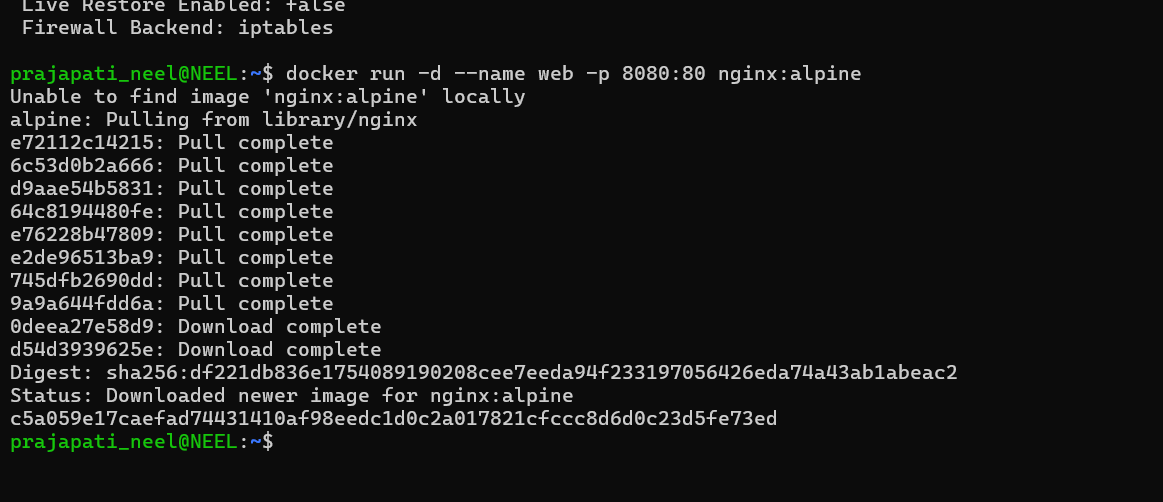
\includegraphics[width=0.85\textwidth]{Screenshot 2026-09-30 132534.png}
    \caption{Running first nginx:alpine container and pulling image layers}
\end{figure}

\begin{figure}[H]
    \centering
    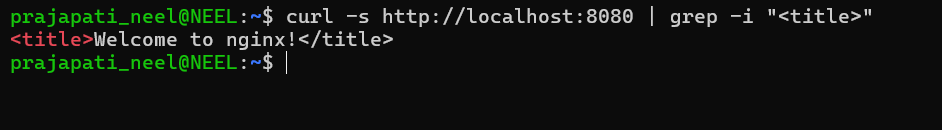
\includegraphics[width=0.85\textwidth]{Screenshot 2026-09-30 132602.png}
    \caption{Verifying nginx container with curl --- ``Welcome to nginx!''}
\end{figure}

\subsection{Verifying with docker ps, docker logs}

Verified the running Nginx container using \texttt{docker ps}, \texttt{docker ps -a}, and \texttt{docker logs web}. The container is up and serving the default Nginx welcome page.

\begin{figure}[H]
    \centering
    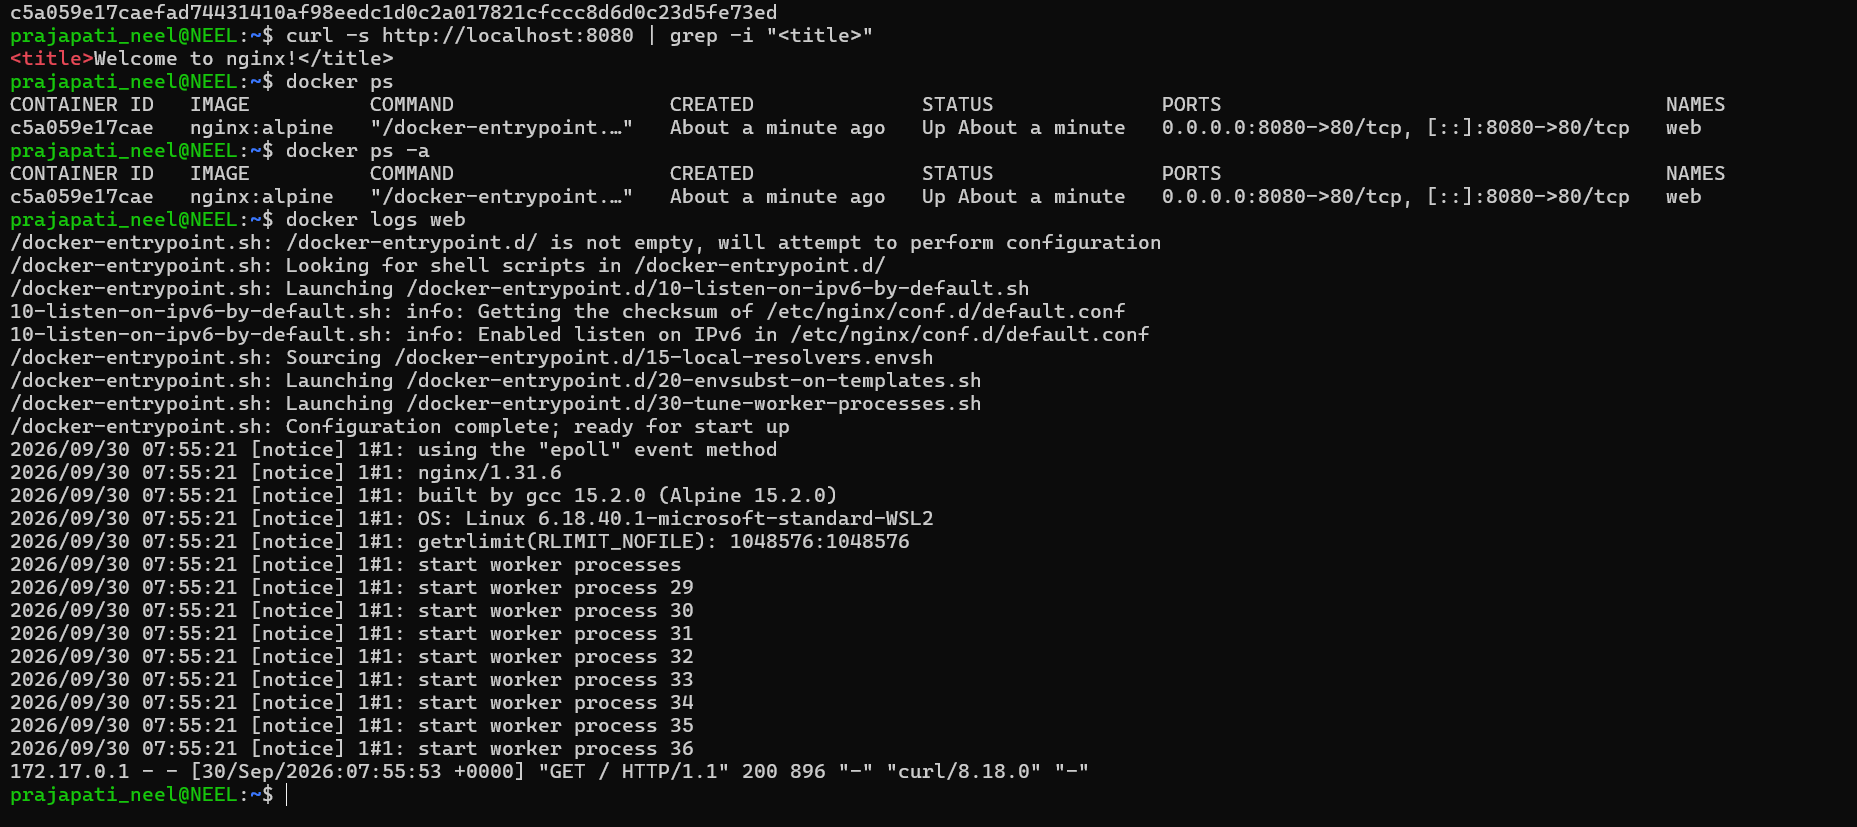
\includegraphics[width=0.85\textwidth]{Screenshot 2026-09-30 132652.png}
    \caption{docker ps, docker ps -a, and docker logs output}
\end{figure}

% ═══════════════════════════════════════════════════════════════════════════
\section{Step 2: Images vs Containers}

\subsection{Pull, Create, Start Stages}

Demonstrated the three stages of \texttt{docker run}: pull (downloading the image), create (preparing the container), and start (running it). Showed that \texttt{docker run = pull + create + start}.

\begin{figure}[H]
    \centering
    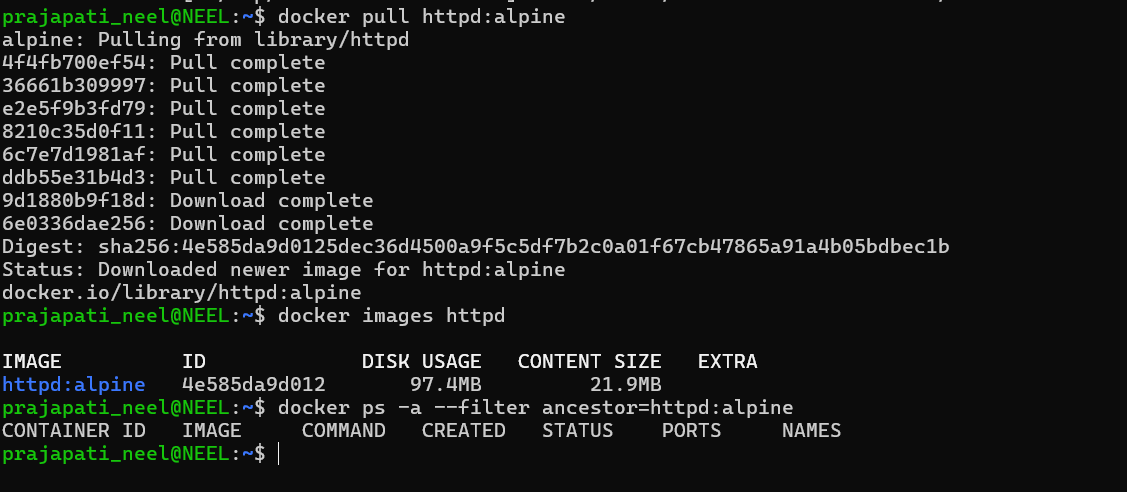
\includegraphics[width=0.85\textwidth]{Screenshot 2026-09-30 132827.png}
    \caption{Pulling httpd:alpine and creating container separately}
\end{figure}

\begin{figure}[H]
    \centering
    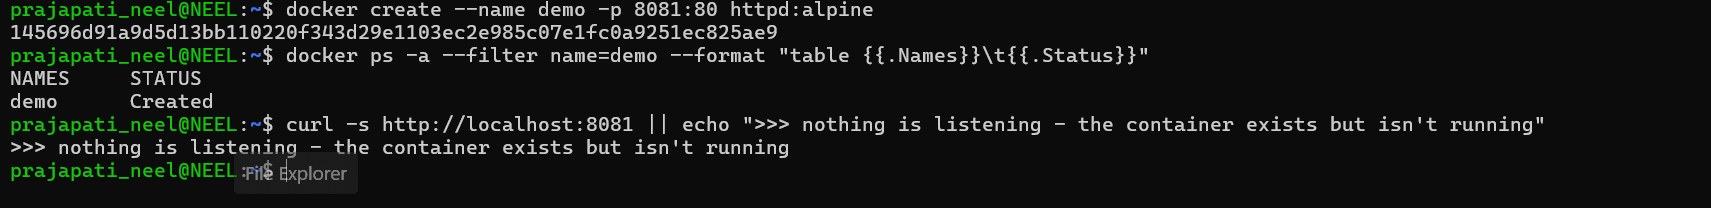
\includegraphics[width=0.85\textwidth]{Screenshot 2026-09-30 132908.png}
    \caption{Starting the container and verifying with curl}
\end{figure}

\subsection{One Image, Many Containers}

Explored creating multiple containers from a single image, container naming conflicts, and the difference between \texttt{docker stop} (polite, 10s timeout) vs \texttt{docker kill} (instant).

\begin{figure}[H]
    \centering
    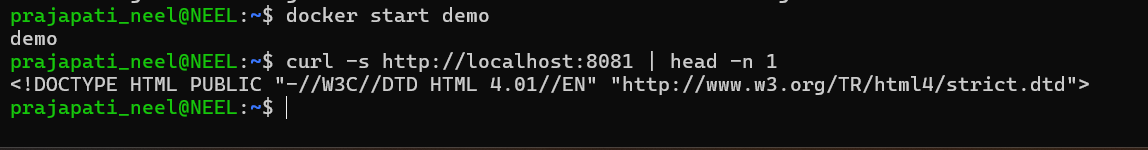
\includegraphics[width=0.85\textwidth]{Screenshot 2026-09-30 132933.png}
    \caption{Multiple containers from one image and stop vs kill timing}
\end{figure}

% ═══════════════════════════════════════════════════════════════════════════
\section{Step 3: Look Inside a Container}

\subsection{Exploring Container Internals}

Used \texttt{docker exec -it web sh} to get a shell inside the container. Observed that the container sees itself as PID 1 with its own hostname and filesystem (Alpine Linux), while sharing the same kernel as the host.

\begin{figure}[H]
    \centering
    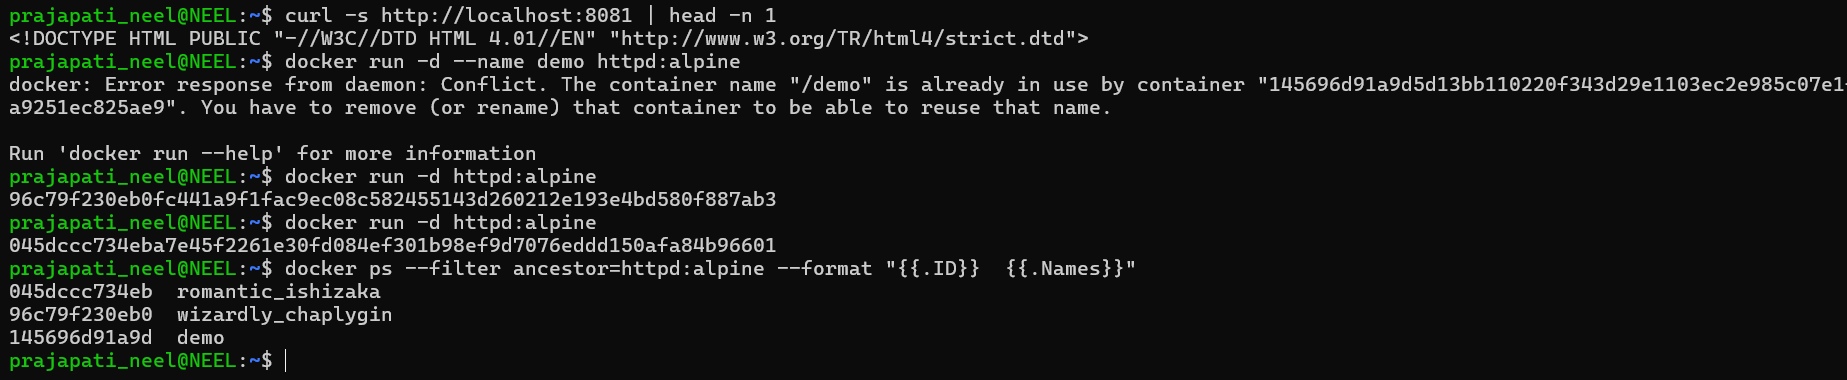
\includegraphics[width=0.85\textwidth]{Screenshot 2026-09-30 133027.png}
    \caption{Inside the container --- hostname, ps, filesystem exploration}
\end{figure}

\begin{figure}[H]
    \centering
    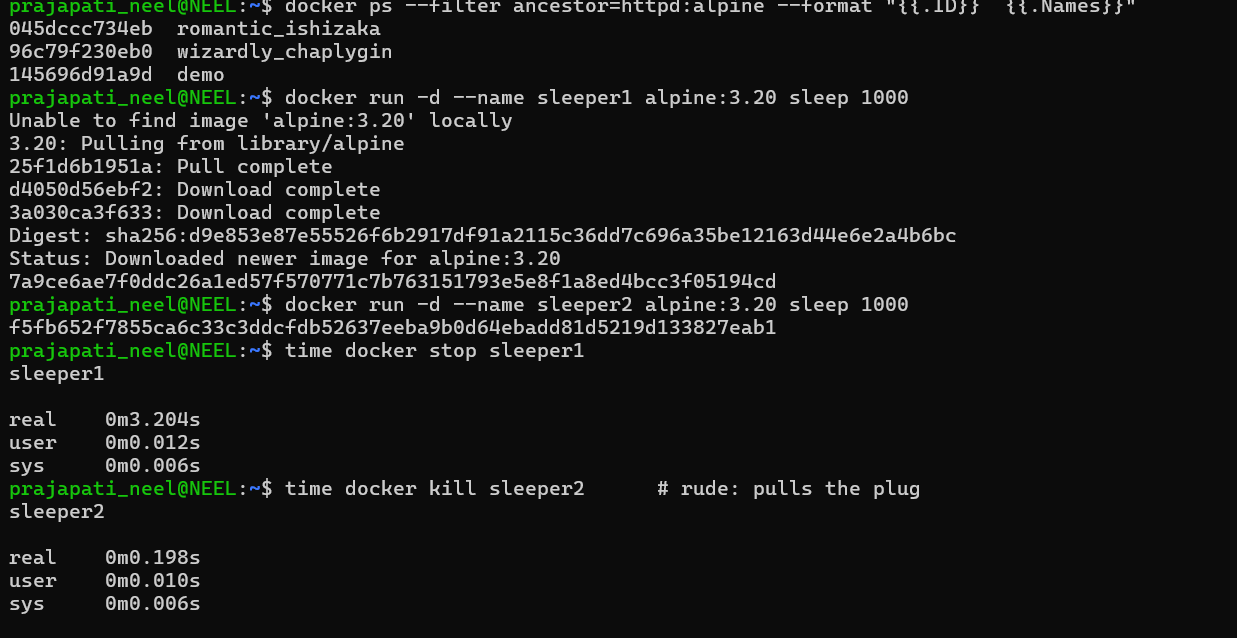
\includegraphics[width=0.85\textwidth]{Screenshot 2026-09-30 133117.png}
    \caption{Proving same kernel --- container uses host's kernel (not a VM)}
\end{figure}

% ═══════════════════════════════════════════════════════════════════════════
\section{Step 4: Who Actually Does the Work?}

\subsection{Docker Architecture}

Explored the Docker architecture by examining \texttt{dockerd}, \texttt{containerd}, and the shim process. Demonstrated starting a container using \texttt{curl} to talk directly to the Docker daemon's REST API via the Unix socket.

\begin{figure}[H]
    \centering
    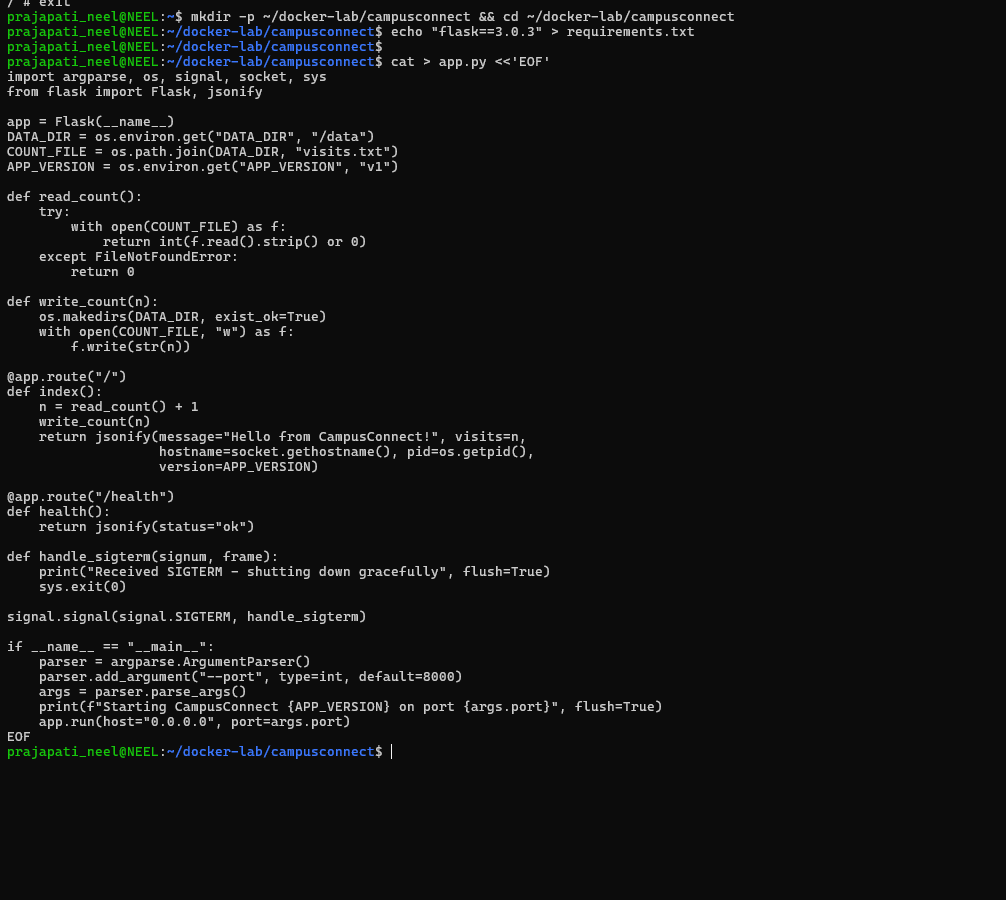
\includegraphics[width=0.85\textwidth]{Screenshot 2026-09-30 134139.png}
    \caption{Creating a container via the Docker API with curl}
\end{figure}

\subsection{Stopping the Daemon}

Stopped the Docker daemon with \texttt{systemctl stop docker} and observed that the CLI could no longer communicate. Restarted the daemon and cleaned up.

\begin{figure}[H]
    \centering
    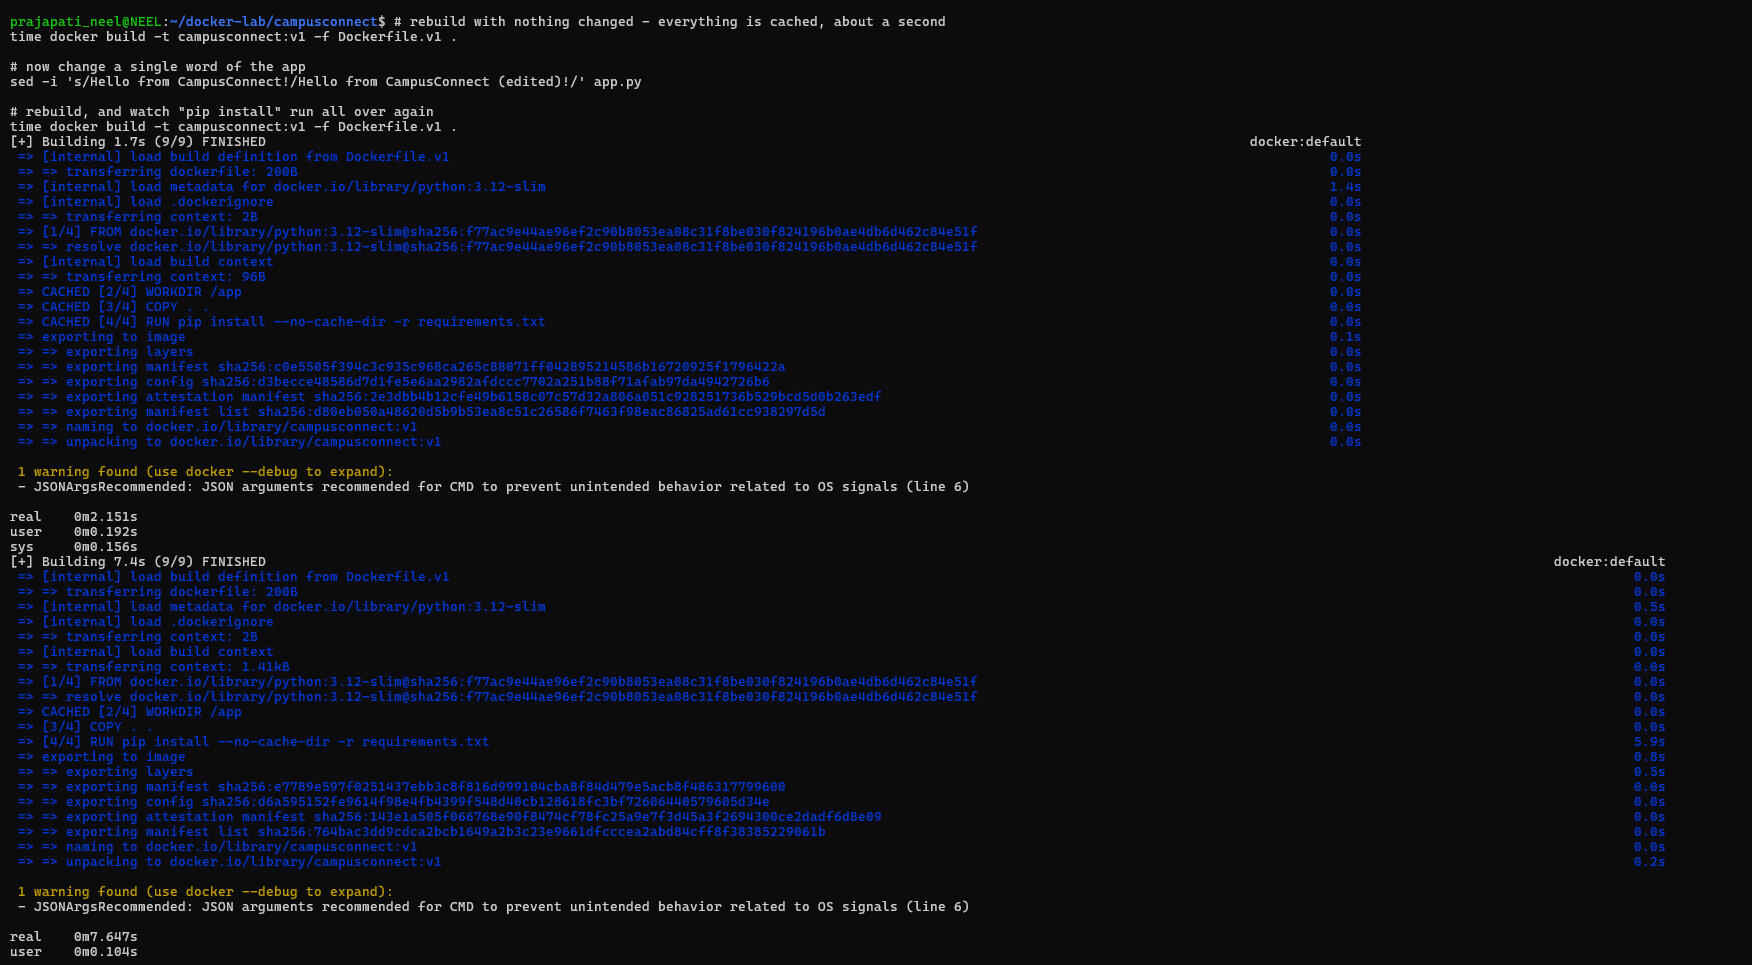
\includegraphics[width=0.85\textwidth]{Screenshot 2026-09-30 134345.png}
    \caption{Daemon stopped --- CLI becomes useless, then restarted}
\end{figure}

% ═══════════════════════════════════════════════════════════════════════════
\section{Step 5: Setting Limits (cgroups)}

CPU and memory limits using cgroups. Created containers with resource limits (\texttt{--cpus=0.5}, \texttt{--memory=128m}). Verified that the kernel enforces these limits by reading cgroup files. Observed a CPU-burning container capped at 50\%.

\begin{figure}[H]
    \centering
    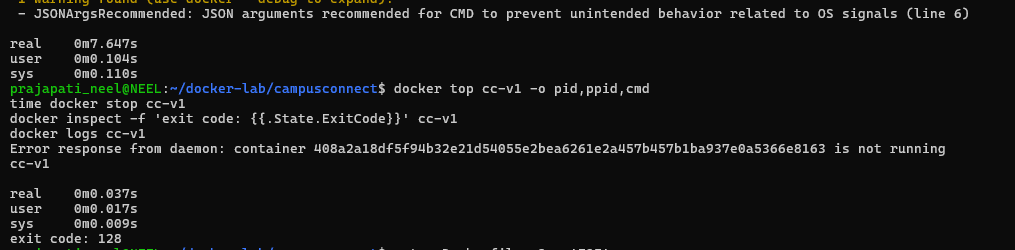
\includegraphics[width=0.85\textwidth]{Screenshot 2026-09-30 134531.png}
    \caption{Setting CPU and memory limits, reading cgroup files}
\end{figure}

\begin{figure}[H]
    \centering
    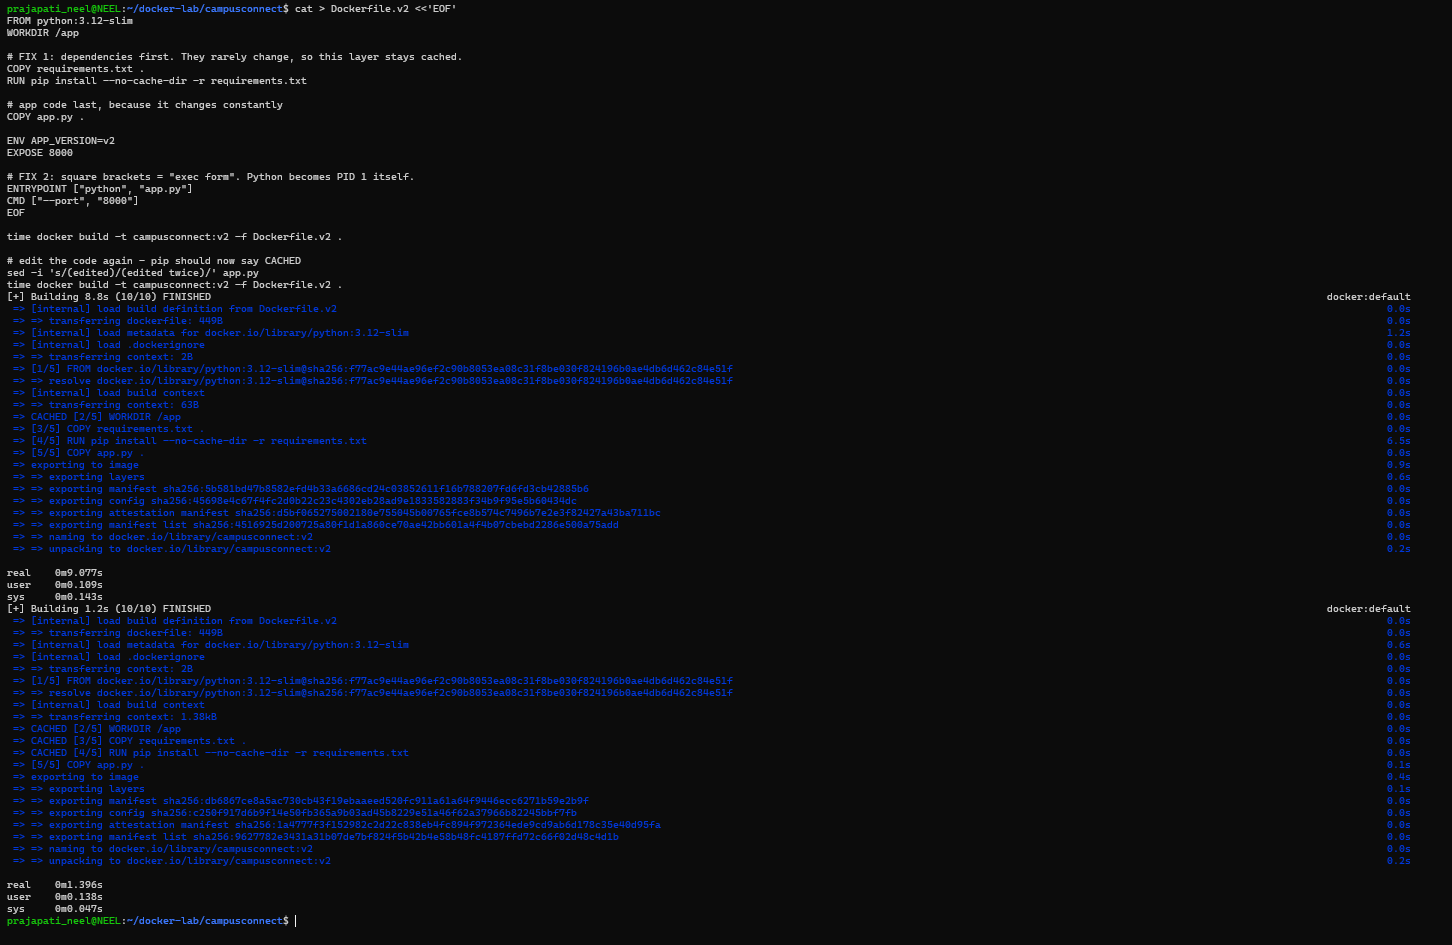
\includegraphics[width=0.85\textwidth]{Screenshot 2026-09-30 134550.png}
    \caption{CPU burner container capped at 50\%, OOM kill test}
\end{figure}

% ═══════════════════════════════════════════════════════════════════════════
\section{Step 6: Layers and Copy-on-Write}

Demonstrated copy-on-write by modifying a file in one container (cow1) and showing that the twin container (cow2) remains unaffected. Verified the thin writable layer cost using \texttt{docker ps -s}.

\begin{figure}[H]
    \centering
    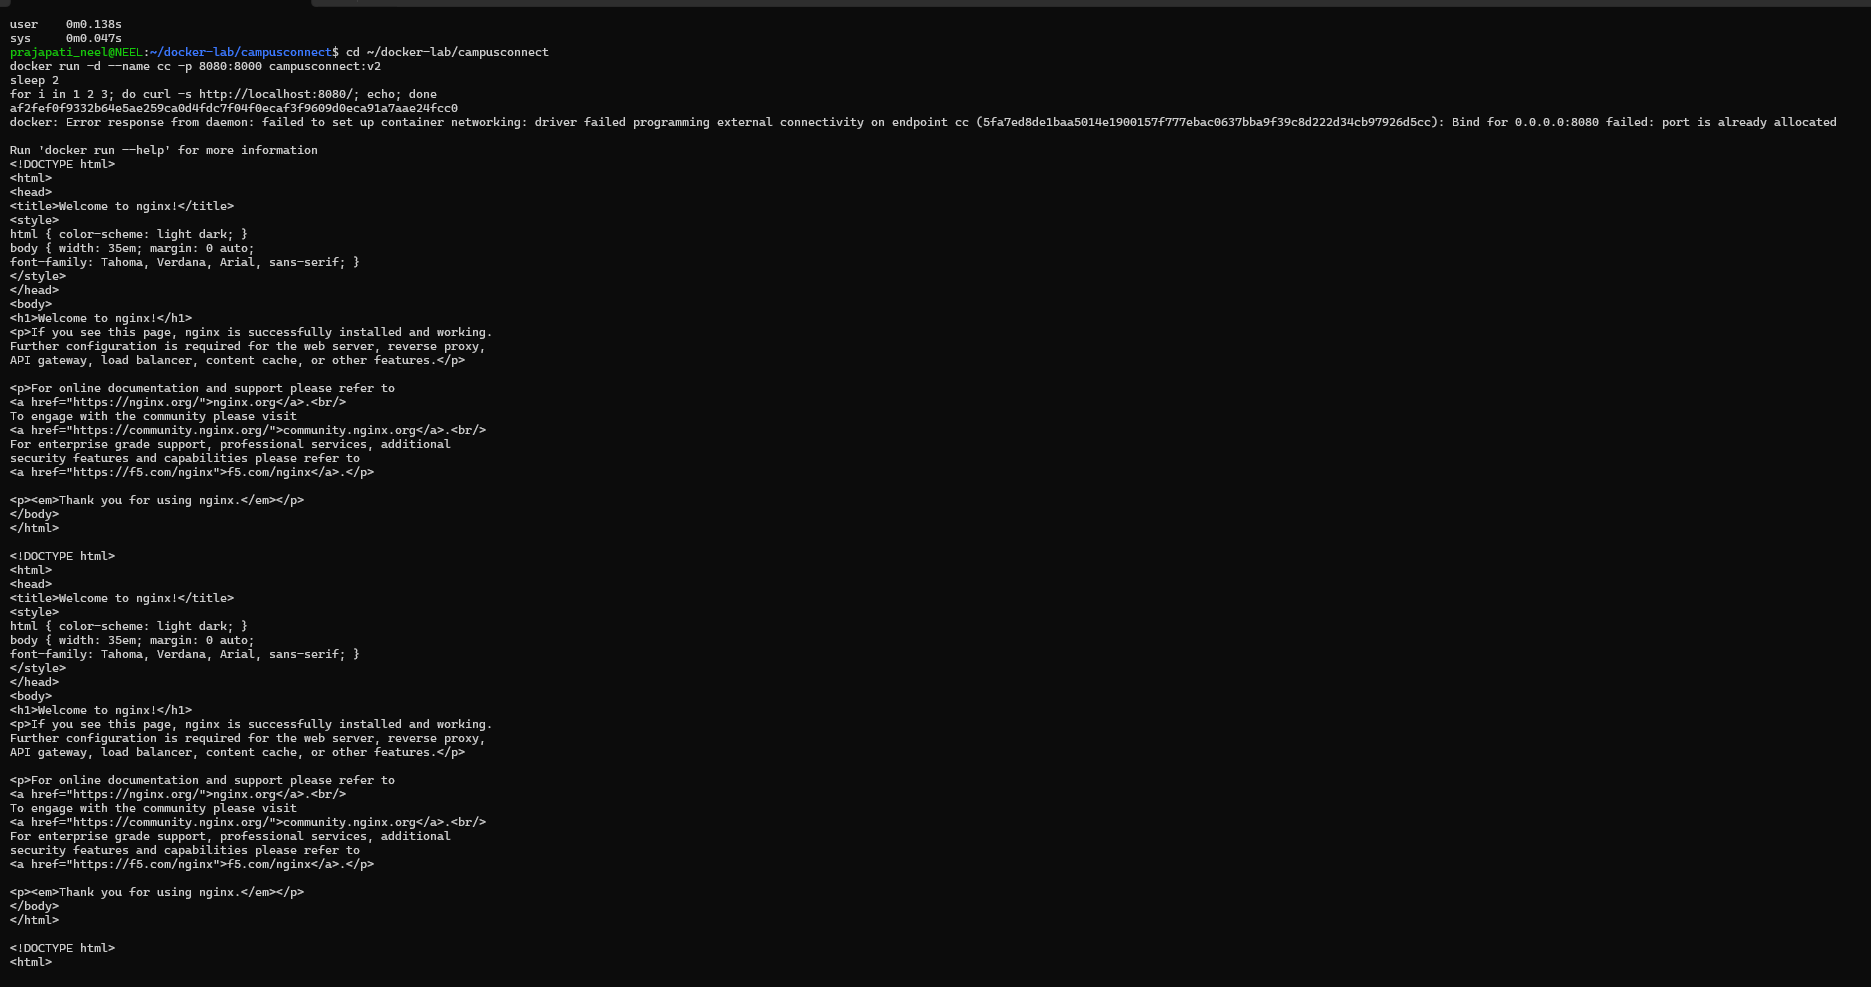
\includegraphics[width=0.85\textwidth]{Screenshot 2026-09-30 134631.png}
    \caption{Copy-on-write: modifying cow1, cow2 stays unchanged}
\end{figure}

\begin{figure}[H]
    \centering
    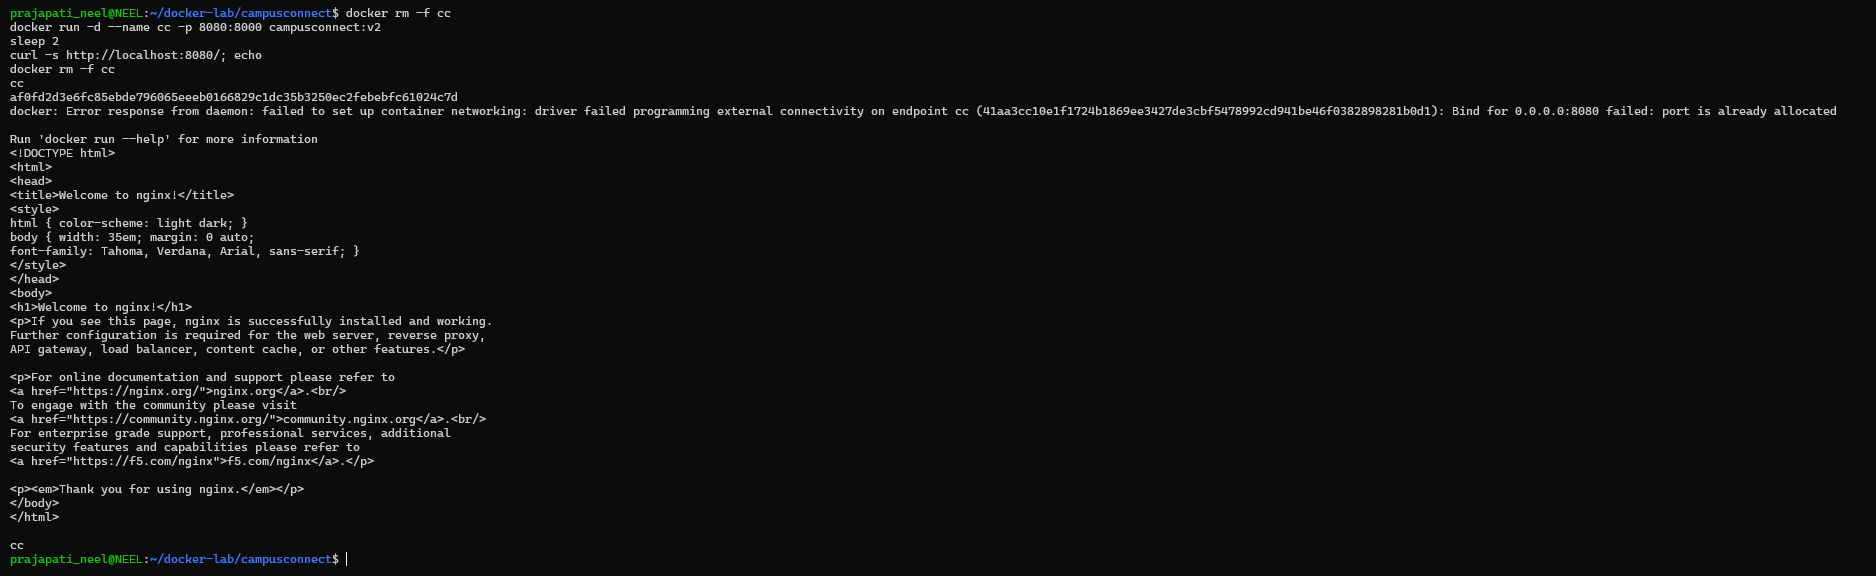
\includegraphics[width=0.85\textwidth]{Screenshot 2026-09-30 134805.png}
    \caption{docker diff and docker ps -s showing layer costs}
\end{figure}

% ═══════════════════════════════════════════════════════════════════════════
\section{Step 7: Build Your Own Image}

\subsection{Writing a Dockerfile for CampusConnect}

Created the CampusConnect visit counter app, wrote \texttt{Dockerfile.v1}, built the image, and ran it. Identified two bugs: slow rebuilds due to poor layer ordering, and shell-form CMD preventing graceful shutdown.

\begin{figure}[H]
    \centering
    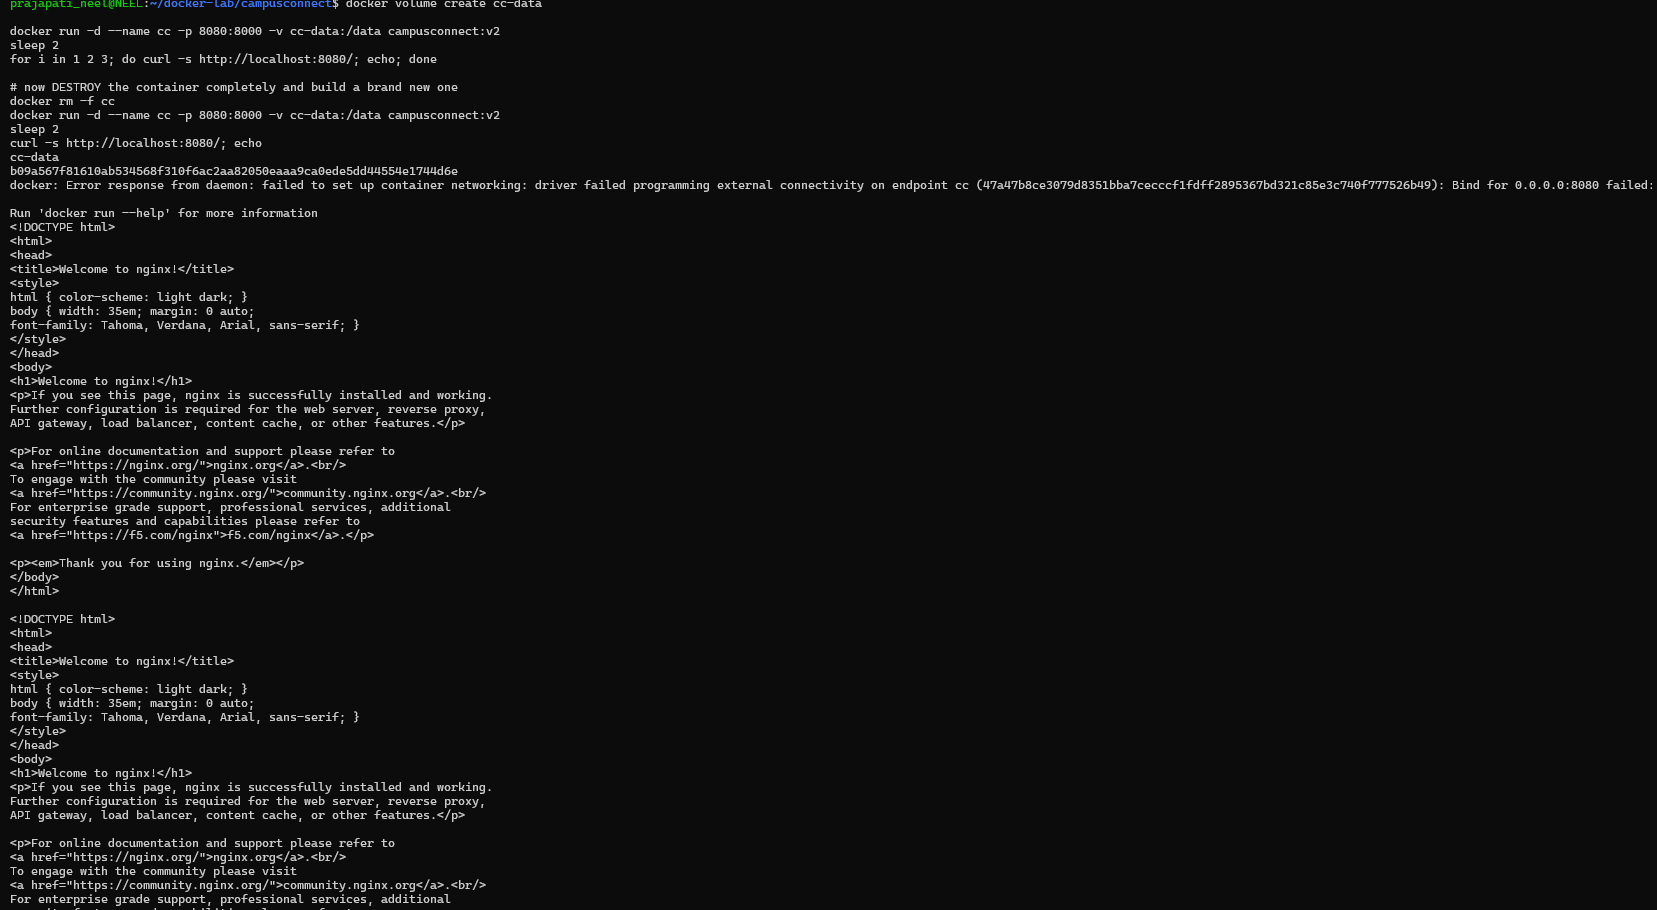
\includegraphics[width=0.85\textwidth]{Screenshot 2026-09-30 134824.png}
    \caption{Building CampusConnect v1 and identifying the shell-form bug}
\end{figure}

\begin{figure}[H]
    \centering
    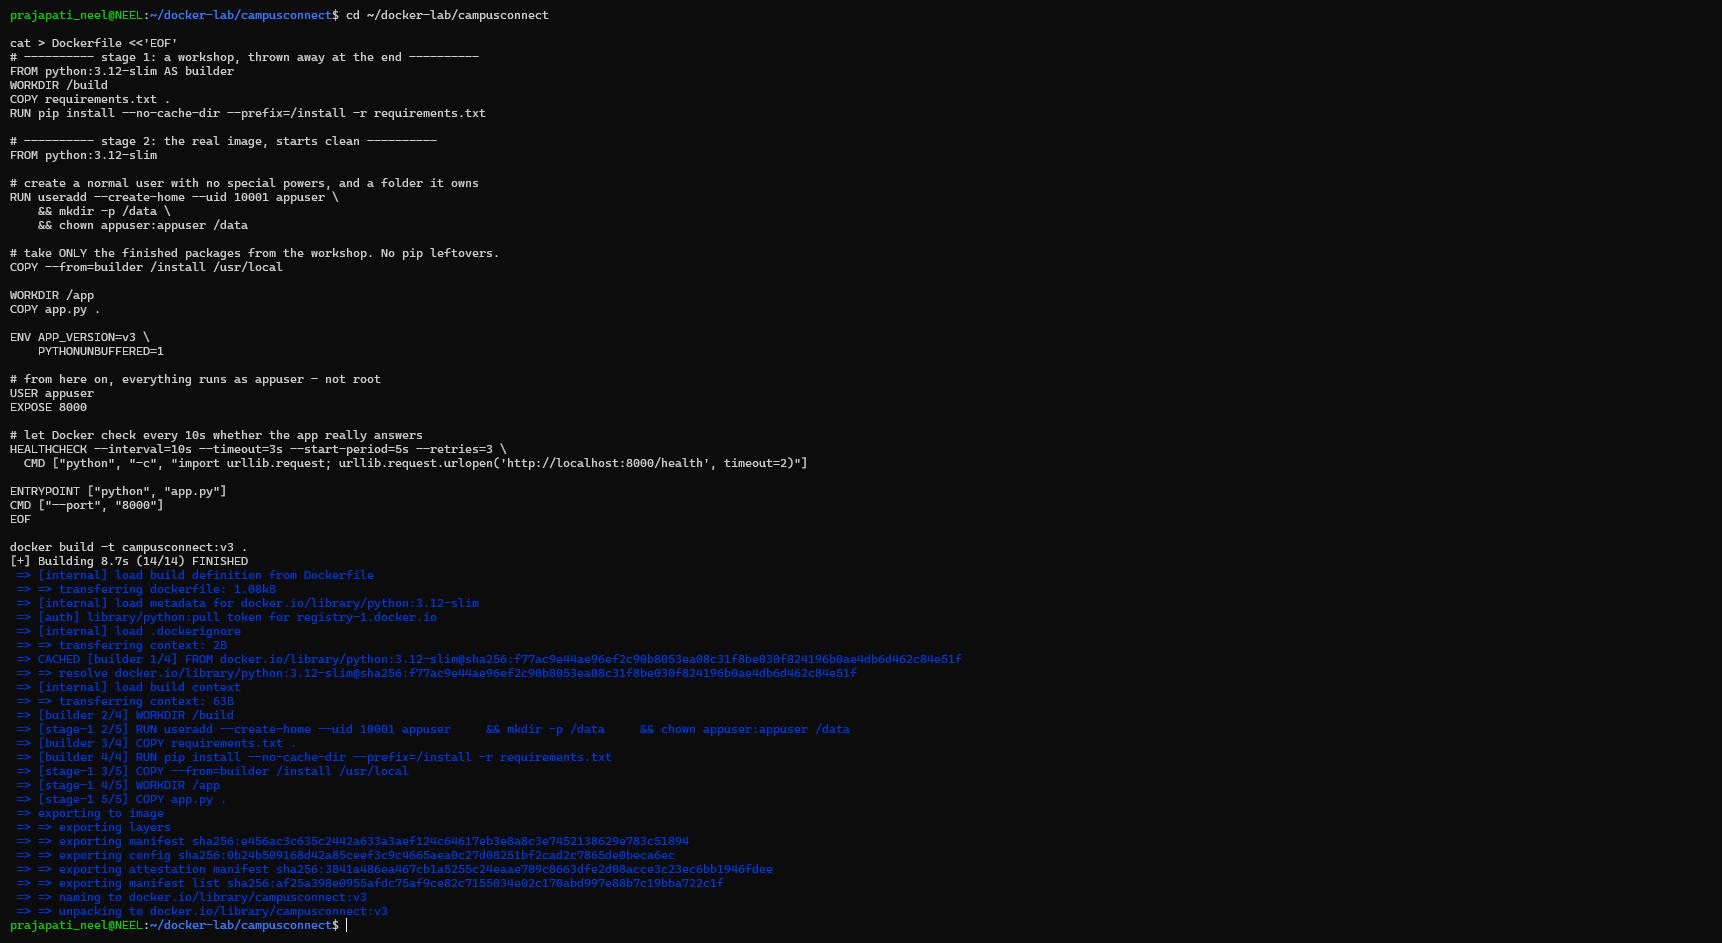
\includegraphics[width=0.85\textwidth]{Screenshot 2026-09-30 134910.png}
    \caption{10-second stop time and exit code 137 --- PID 1 problem}
\end{figure}

\subsection{Fixing the Dockerfile}

Created \texttt{Dockerfile.v2} with fixes: dependencies copied before app code (for cache efficiency), and exec-form ENTRYPOINT so Python becomes PID 1 and receives SIGTERM properly. Verified graceful shutdown.

\begin{figure}[H]
    \centering
    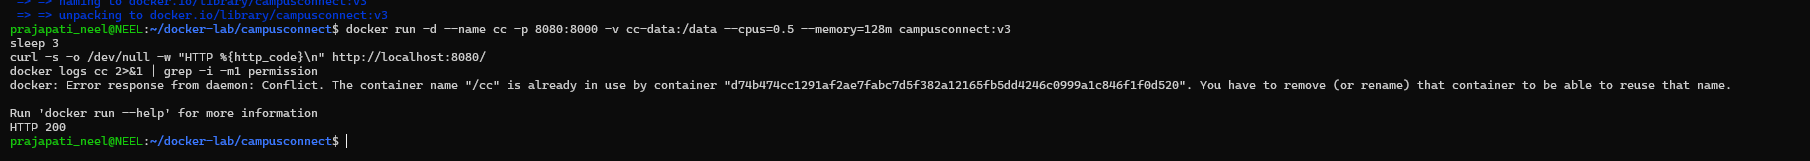
\includegraphics[width=0.85\textwidth]{Screenshot 2026-09-30 134927.png}
    \caption{v2 with exec-form: clean shutdown in 0.2s, exit code 0}
\end{figure}

\begin{figure}[H]
    \centering
    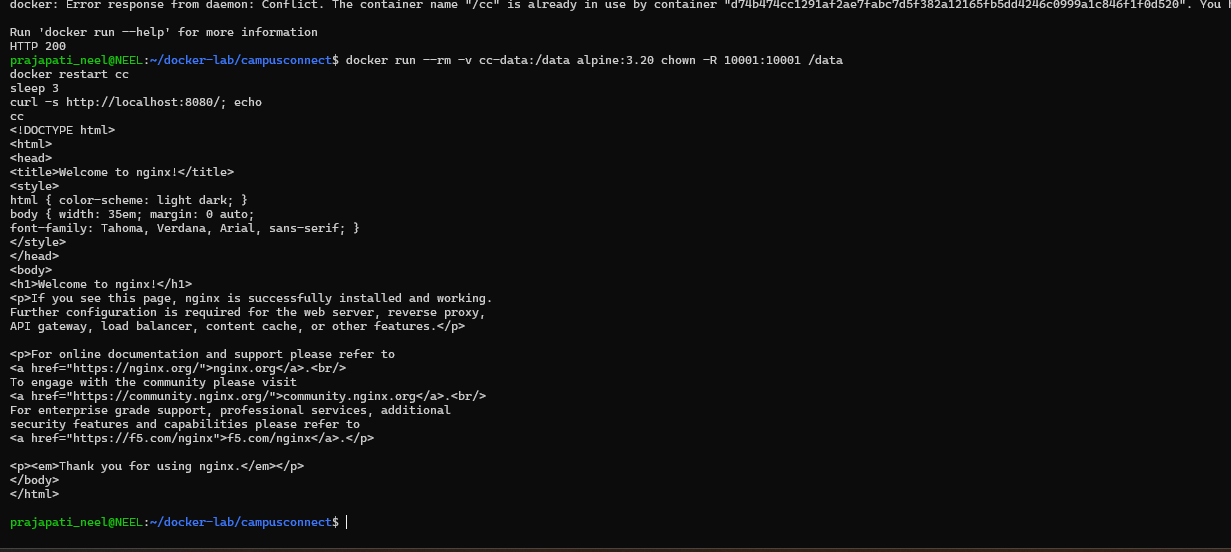
\includegraphics[width=0.85\textwidth]{Screenshot 2026-09-30 134947.png}
    \caption{SIGTERM received gracefully --- ``Received SIGTERM'' in logs}
\end{figure}

% ═══════════════════════════════════════════════════════════════════════════
\section{Step 8: Keep Your Data (Volumes)}

Demonstrated data loss when containers are deleted. Fixed it using Docker volumes (\texttt{docker volume create cc-data}) and bind mounts. Showed that the visit counter persists across container recreations.

\begin{figure}[H]
    \centering
    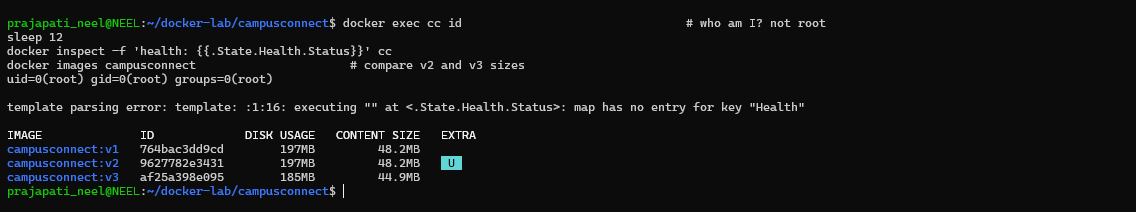
\includegraphics[width=0.85\textwidth]{Screenshot 2026-09-30 135014.png}
    \caption{Volume mount --- data persists across container deletion}
\end{figure}

\begin{figure}[H]
    \centering
    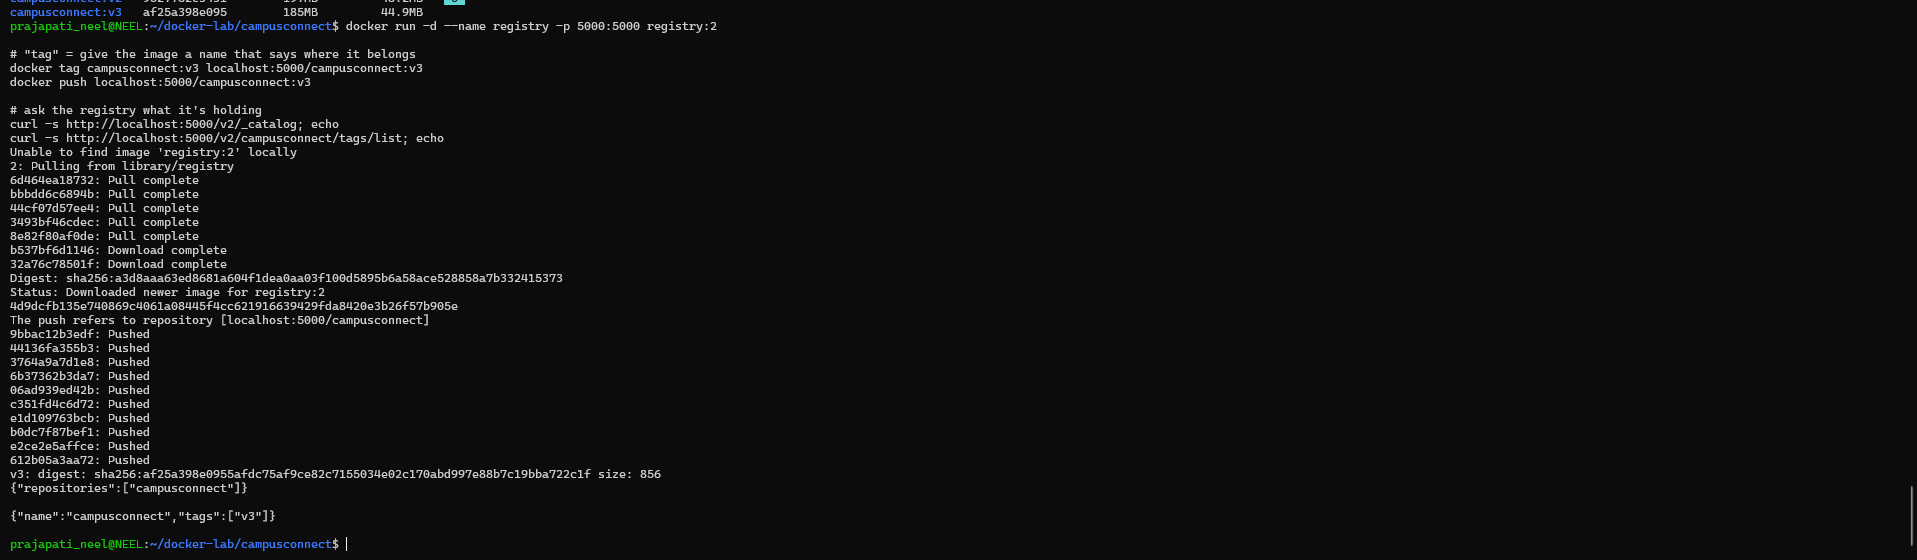
\includegraphics[width=0.85\textwidth]{Screenshot 2026-09-30 135045.png}
    \caption{Bind mounts and volume inspection}
\end{figure}

% ═══════════════════════════════════════════════════════════════════════════
\section{Step 9: Ship It Like a Pro}

Built a production-ready Dockerfile with multi-stage build, non-root user (\texttt{appuser}), and HEALTHCHECK. Published the image to a local Docker registry and pulled it back for deployment.

\begin{figure}[H]
    \centering
    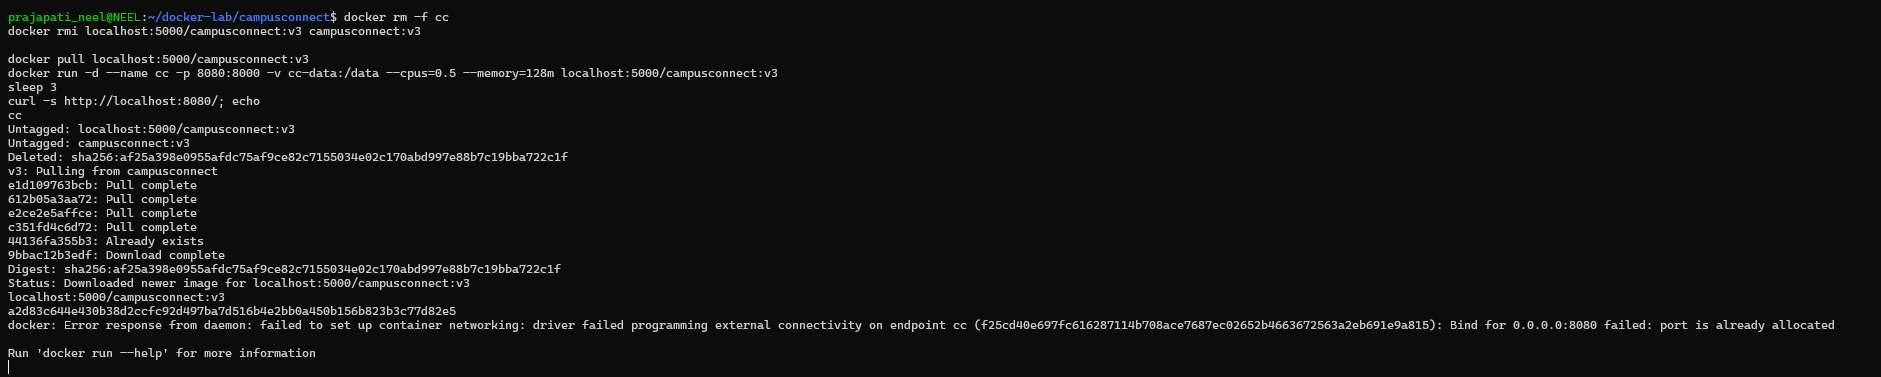
\includegraphics[width=0.85\textwidth]{Screenshot 2026-09-30 135101.png}
    \caption{Multi-stage build, non-root user, and health check}
\end{figure}

\begin{figure}[H]
    \centering
    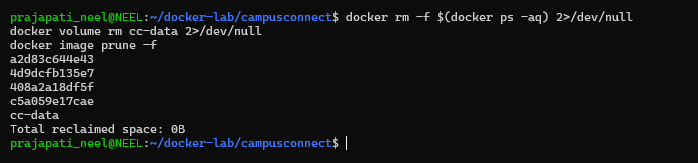
\includegraphics[width=0.85\textwidth]{Screenshot 2026-09-30 135113.png}
    \caption{Pushing to local registry and pulling back for deployment}
\end{figure}

% ═══════════════════════════════════════════════════════════════════════════
\section{Conclusion}

This hands-on lab provided comprehensive practical experience with Docker containerization. Through the nine steps, the following key learnings were achieved:

\begin{enumerate}[nosep]
    \item A container is a single process wrapped with kernel namespaces and cgroups --- not a virtual machine. It shares the host's kernel and starts in a fraction of a second.

    \item \texttt{docker run} is a convenience shortcut for \texttt{pull + create + start}. Understanding this decomposition is essential for advanced usage and API-based automation.

    \item Inside a container, the main process is PID 1. Outside, it appears as a regular process in the host's process list --- same kernel, different view (namespaces).

    \item The Docker CLI is just a client that sends HTTP requests to the Docker daemon (\texttt{dockerd}) over a Unix socket. The daemon delegates to \texttt{containerd}, which uses \texttt{runc} to create containers.

    \item Cgroups provide resource limits (CPU, memory). Exit code 137 indicates a force-kill, often due to OOM or ignored SIGTERM.

    \item Images consist of shared read-only layers. Each container adds a thin writable layer (copy-on-write), making containers extremely lightweight.

    \item Dockerfile best practices: place rarely-changing instructions first (dependencies before code), and always use exec-form (square brackets) for ENTRYPOINT/CMD so the application receives signals properly.

    \item Volumes provide persistent storage that survives container deletion. Bind mounts allow direct access to host filesystem directories.

    \item Production images should use multi-stage builds, run as non-root users, include health checks, and be published to a registry for deployment.
\end{enumerate}

The lab successfully demonstrated the complete Docker workflow: from running a first container to building, optimizing, and publishing a production-ready image.

\end{document}
